\section{Geometric Deep Learning}
\subsection{Sets \& Points}
Goal: realize some function \(\{x_1,\ldots, x_M\}\subset R,\quad f:2^R\rightarrow \mathcal{Y}\). 
Naively, we could turn the set into an ordered N-tupel \(\{x_1, \ldots, x_M\} \mapsto (x_1,\ldots, x_M)\in R^M\) and then apply standard DNN \(\leadsto\) Problems: variable-length inputs if sets have different cardinality \& arbitrariness of ordering of elements\\
\textbf{Invariance and Equivariance:} 
\begin{enumerate}
    \item \(f\) is \textit{order-invariant} iff \(f(x_1, \ldots, x_M)=f(x_{\pi_1}, \ldots, x_{\pi_M})\, \bm{x}\in R^M,\forall \pi \in S_M\), \(\pi:\) permutation, \(S_M\): symmetric group
    \item \(f\) is \textit{order-equivariant} iff \(f(x_1,\ldots x_M)=(y_1,\ldots, y_M)\implies f(x_{\pi_1},\ldots, x_{\pi_M})=(y_{\pi_1},\ldots, y_{\pi_M})\, \bm{x}\in R^M,\forall \pi\in S_M\)
\end{enumerate}
More general, for some transformation \(T\in \mathcal{T}\), where \(\mathcal{T}\) is some group of transformations, and a function \(f\), we call \(f\)
\begin{enumerate}
    \item \textit{invariant} iff \(f(T(x_1,\ldots, x_M))=f(x,\ldots, x_M)\, \forall \bm{x}\in R^M,\forall T\in \mathcal{T}\)
    \item \textit{equivariant} iff \(f(T(x_1,\ldots, x_M))=T(f(x_1, \ldots, x_M))\, \forall \bm{x}\in R^M, \forall T\in \mathcal{T}\)
\end{enumerate}
Examples: conv. operator is equivariant to translations; att. mechanism permutation equivariant with regard to token sequence since softmax is equivariant operation; Euclidean norm is invariant under rotations

\textbf{Deep Sets:}
\begin{itemize}
    \item Sum is invariant under permutations (commutativity): \(\sum_{m=1}^M x_m = \sum_{m=1}^M x_{\pi_m},\, \forall M, \forall\pi\in S_M\)
\(\leadsto\) by allowing for other (fixed or DNN) maps \(\phi:R \rightarrow \mathbb{R}^N\) and \(\rho: \mathbb{R}^N  \rightarrow \mathbb{R}\) we can construct a larger class of invariant function as follows: 
\(f(x_1, \ldots x_M)=\rho\left(\sum_{m=1}^M \phi(x_m)\right),\) where \(\phi, \rho\) are independent of \(M\), so \(f\) is defined over an arbitrary number of inputs. 
    \item Can construct invariant mappings using different agg. functions such as (point-wise) max.\& min., etc.: \(f(x_1, \ldots, x_M)=\rho\left(\max_{m=1}^M \phi(x_m)\right)\)
    \item Once we have invariant \(f\), this can be turned into an equiv. map using \(\rho: R\times \mathbb{R}^N \rightarrow \mathcal{Y}, \, \left(x_m, \sum_{k=1}^M \phi(x_k)\right) \mapsto y_m\) and apply pointwise for each \(x_m\). Hence, the down-stream processing \(\rho\) depends on an invar. argument (here: aggregated as sum) and \(x_m\) itself (via shortcut connection)
    \item fixed \(N\) (width of hidden representations) is sufficient if one allows for discontinuous mappings in the limit of \(M \rightarrow \infty\), but more practically realizable mappings may require \(N\geq M\)
\end{itemize}

\textbf{PointNet:} Sparse measurements at specific 3D points i.e. point cloud \(\leadsto\) desirable that a DNN obeys permutation in-/equivariance
%\vspace{-1em}
%\begin{center}
%    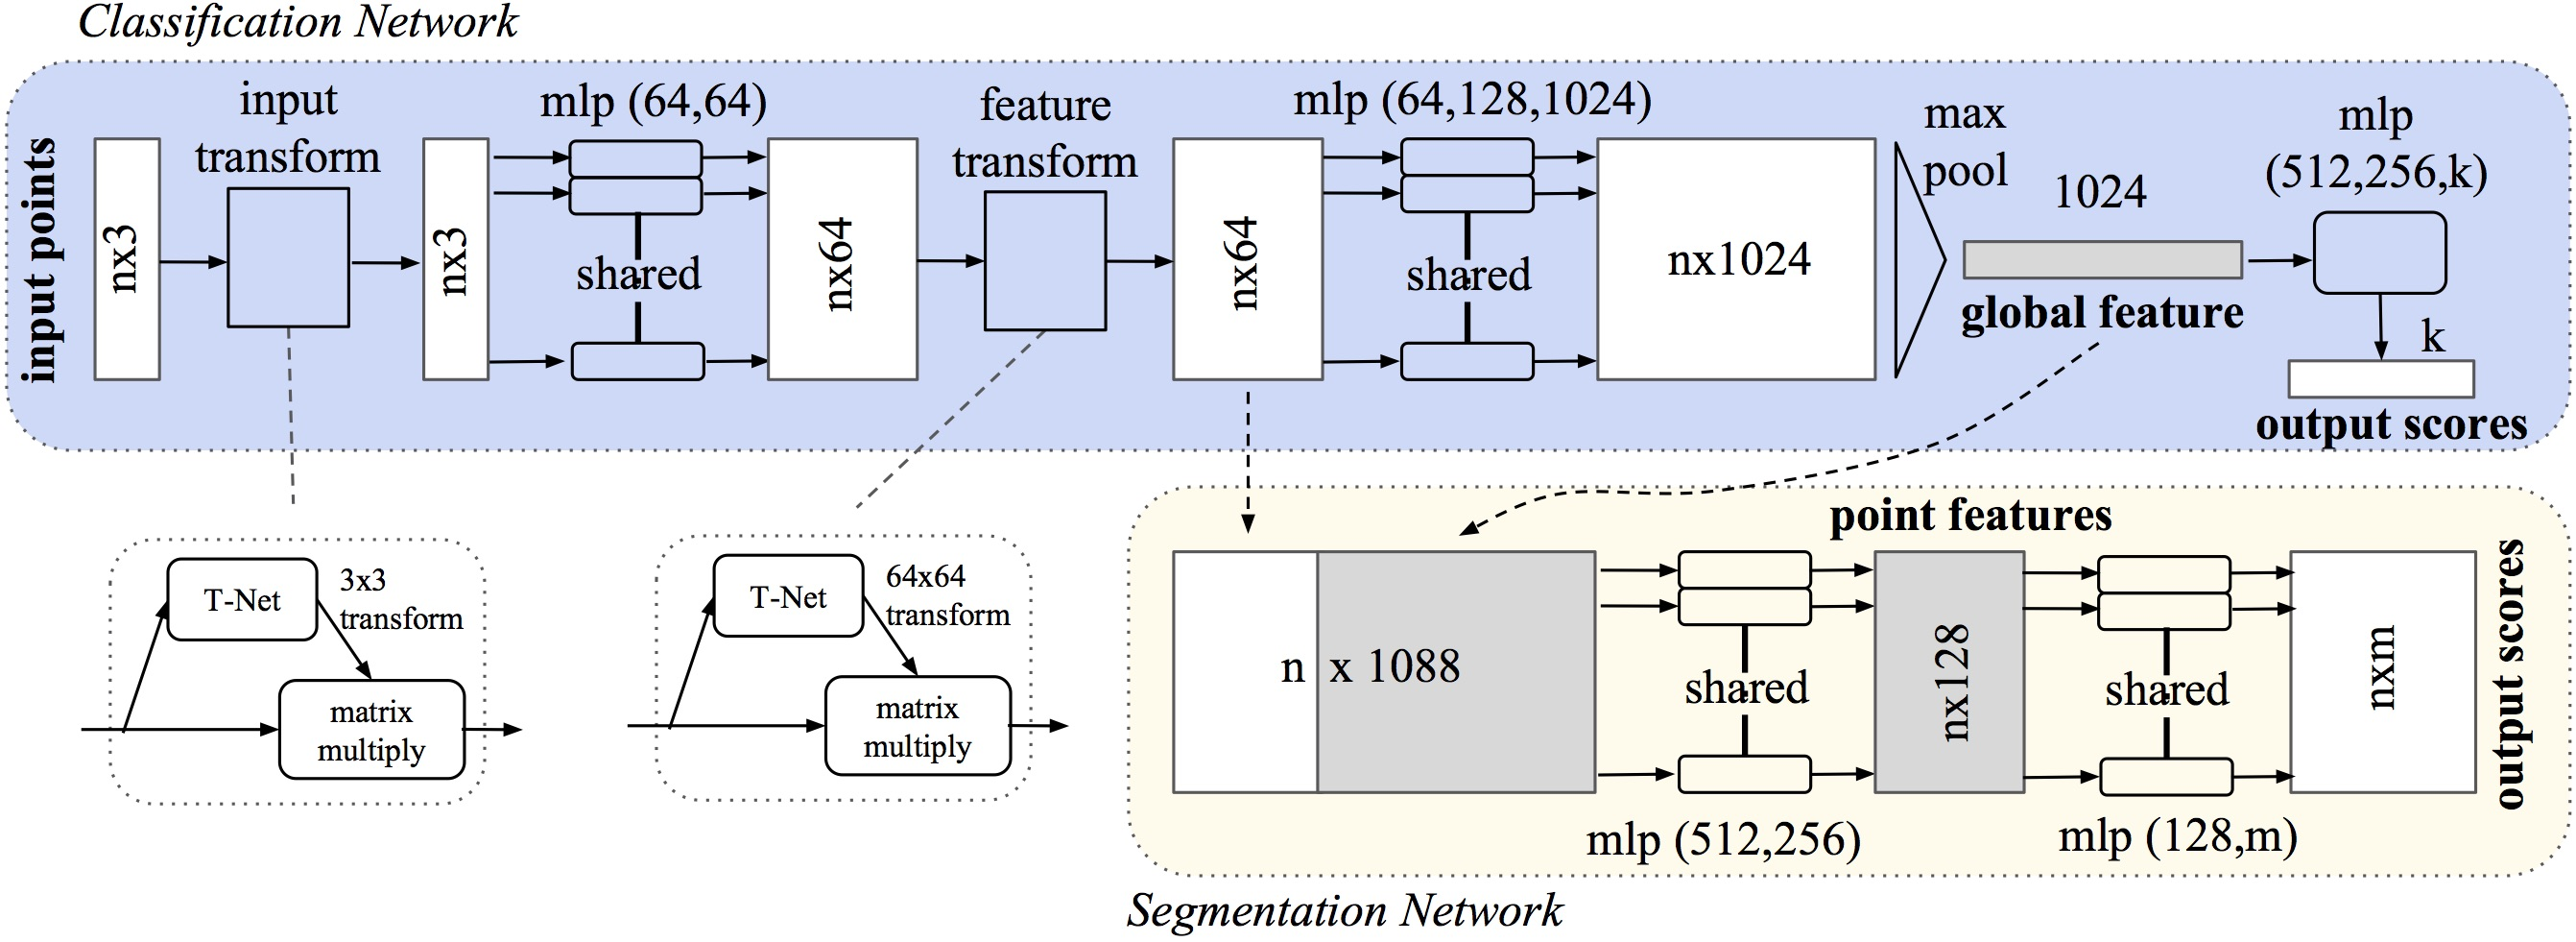
\includegraphics[scale = 0.05]{contents/imgs/pointnet.jpg}
%\end{center}
\subsection{Graph Convolutional Networks}
\textbf{Basics:} Set of Vertices \(\mathcal{V}=\{v_1, \ldots, v_M\}\). We associate a feature vector \(x_m\) with every node and consider undirected edges \(\mathcal{E}=\{e_1, \ldots, e_K\}\subseteq \{e\in 2^V: |e|=2\}\). Idea: graph may encode similarities between nodes and corresponding dependencies between their outputs.\newline
\textbf{Adj. Matrix: } \(A=(a_{nm}), \quad a_{nm} = \mathbb{I}_{\{v_n, v_m\}\in \mathcal{E}}\). A is symmetric and has 0 diagonal (i.e. no self-loops)\newline
\textbf{Permut. Matrix:} \(P \in \{0, 1\}^{M\times M}\, \text{s.t.} \, \sum_{n=1}^M p_{nm}=\sum_{n=1}^M p_{mn} = 1 \, \forall m\) Cauchy's two line notation for permutations: \(P = \begin{pmatrix}
    0 & 0 & 1 & 0 \\
    0 & 1 & 0 & 0 \\
    0 & 0 & 0 & 1 \\
    1 & 0 & 0 & 0
    \end{pmatrix}
    \quad \leftrightarrow \quad
    \begin{array}{l}
    \pi = \begin{pmatrix}
    1 & 2 & 3 & 4 \\
    3 & 2 & 4 & 1
    \end{pmatrix} ;\quad
    \pi^{-1} = \begin{pmatrix}
    1 & 2 & 3 & 4 \\
    4 & 2 & 1 & 3
    \end{pmatrix}
    \end{array}
\)
\(\pi \& \pi^{-1}\) are always inverse elements in the group \(S_M\)\newline
Permutation matrices are orthogonal i.e. \(P^{-1} = P^{\prime} \, \text{or} \, PP^{\prime}=P^{\prime}P = I \, \text{as} \, (PP^{\prime})_{nm}=\sum_{k}p_{nk}p_{mk}=\delta_{nm}\)
Let \(\Pi_M\) be the group of permutation matrices, then invar. of a function of a graph can be defined as \(f(X,A)\stackrel{!}{=} f(PX, PAP^{\prime}),\, \forall P \in \Pi_M\) and equiv. as \(Pf(X, A) \stackrel{!}{=} f(PX, PAP^{\prime}),\, \forall P \in \Pi_M\)\newline
\textbf{Invariant Core:} Multiset of features in neighborhood of node \(i\): \(X_m=\{\{x_n: \{v_n, v_m\} \in \mathcal{E}\}\}, \, \{\{\}\}= \text{multiset}\) i.e. for given node \(v_m\)it's the multiset of feature vectors from its neighbors. Choose any \(\phi: (x_m, X_m)\mapsto \phi(x_m, X_m)\in \mathbb{R}^N\). We can then apply this function at every node to arrive at \(X \mapsto \phi(X) := \begin{pmatrix}
        \phi(x_1, X_1)^{\prime} \\
        \vdots \\
        \phi(x_M, X_M)^{\prime}
    \end{pmatrix}
 \in \mathbb{R}^{M \times N}\)\newline
 Note that any pair of isomorphic graphs (i.e. graphs that are bijective under edge re-numbering) are processed in the same manner. \(\phi\) can be designed e.g. by transforming node features and then aggregating by summation: \(\phi(x_m, X_m) = \phi(x_m, \sum_{x\in X_m} \psi(x))\). If globally invariant function is desired, one can add a final invariant aggregation step.
\textbf{Graph-Learning Scenarios:} \textit{node classification}: make a discrete/real-valued prediction at every node; \textit{graph classification}: classify the entire graph; \textit{link prediction}: predict missing edges in graph

\textbf{Coupling Matrix:} In convolutional graph NNs, the aggregation over neighborhoods is performed with a fixed sets of weights known as coupling matrix (typically derived from adj. matrix A). Often we add self-loops to A and normalize with the degree matrix as follows: \(\bar{A} = D^{-1/2} (A+I)D^{-1/2}, \, D = \diag(d_1, \ldots, d_M),\, d_m = 1+\sum_{n=1}^M a_{nm}\). Rmk: The normalization balances out degree variability between the nodes but the activation of a node propagates to its neighbors. E.g. for a 1-dim (cyclic) chain, a regular graph of degree 2, then \(\bar{A}=1/3 A\)

\textbf{GCN Layers:} Let \(W\) be weight matrix and \(\sigma\) an activation function. Then, one step of propagation in a convolutional GNN: \(Z = \sigma(\bar{A}XW), \, W\in \mathbb{R}^{N\times d}\). Note: Multiplication by \(\bar{A}\) from the left sums over nodes, based on the edge structure of the graph, whereas multiplication by W from the right sums over features. Iteratively, we have for two-layer GCN: \(Z = \softmax(\bar{A} \relu(\bar{A}XW)W_1)\)\\
\textbf{!} Control the spectrum of the coupling matrix \(\bar{A}\): want \(|\lambda(\bar{A})|\leq 1,\) \textrightarrow guarantees stability in terms of repeated propagation in a deep GCN

\textbf{Limitations of GCN:} GCNs require that depth is equal to diameter of graph to propagate between all pairs of nodes \(\leadsto \text{deep networks} \leadsto \text{issues}:\)
\begin{itemize}
    \item \textbf{Oversmoothing:} Repr. at nodes may become indistinguishable
    \item \textbf{Oversquashing:} Bottleneck effect of how much long-range information can be encoded in fixed-size representation \(\leadsto\) can improve learning from long-range dependencies by modyfiying the graph structure to allow for smaller diameters
\end{itemize}

\subsection{Spectral Graph Theory:}
\textbf{Laplacian Operator:} is \(\Delta f:= \sum_{n=1}^N \pd{f^2}{x_n^2}, \, f:\mathbb{R}^N \rightarrow \mathbb{R}\). Think of Laplace operator at \(x\) as measuring local variation from \(f\)-average in a vanishingly small neighborhood of \(x\): for balls of radius \(h\rightarrow 0 \quad \bar{f}(x,h)-f(x)=\dfrac{h^2}{2n}\Delta f(x) + o(h^2)\)\\
\textbf{Graph Laplacian: } with adjacency matrix \(A\) \& degree matrix D: \(L := D-A, \, (Lx)_n = \sum_{m=1}^M a_{nm}(x_n-x_m)\); but in practice often better to use (symmetric) degree-normalized Laplacian: \(\tilde{L}=I-D^{-1/2}AD^{-1/2}=D^{-1/2}(D-A)D^{-1/2}\). Note: \(L\& \tilde{L}\) are symmetric, positive semi-definite and weakly diagonally dominant i.e. \(d_n=\sum_m a_{nm}=\sum_m |a_{nm}|\) \\
\textbf{Graph Fourier Trafo:} \(L=D-A = U\Lambda U^{\prime}, \, \Lambda := \diag(\lambda_1, \ldots, \lambda_M), \, \lambda_i \geq \lambda_{i+1}\) with \(U\) orthogonal. The columns of \(U\) can be considered to be the graph Fourier basis.
\textbf{Graph Convolution: } Pointwise multiplication in the Fourier domain: \(x * y = U((U^{\prime}x) \odot (U^{\prime }y))\). The filtering operation from 1d-signals can be generalized: \(G_{\theta}(L)x = U G_{\theta}(\Lambda) U^{\prime}x \leadsto \mathcal{O}(M^3)\) since full eigendecomposition of \(L\). \textbf{TRICK: Polynomial Kernels} i.e. \(U\left(\sum_{k=0}^K \alpha_k \Lambda^k\right ) U^{\prime}=\sum_{k=0}^K \alpha_k L^k\). If \(A\) sparse (\(\implies L\) sparse), then highly efficient scaling of arithmetic operations with \(|\mathcal{E}|\) as only powers of Laplacian have to be calculated. Spectral conv. can then be expressed as multiple equivariant local layers in the vertex domain. Polynomial order \(K\) defines size of neighborhood (typically 2-5). These filters are isotropic and have fewer params. and lower express. than in traditional convs.\\
\textbf{Polynomial Kernel Networks:} Channel indices denoted by \(i, j\), then pre-activation of graph-convolutional layer can be written as \(x_i^{l+1}=\sum_j p_{ij}(L) x_j^l + b_i, \, p_{ij}(L) = \sum_{k=0}^K \alpha_{ijk}L^k.\) The number of parameters is essentially (ignoring \(b_i\)) the product of the channel dimensions times \(K+1\).

\subsection{Attention GNNs}
\textbf{Coupling with Attention: } Define a coupling matrix via attention: \(Q=(q_{ij}), \, q_{ij} = \softmax(\rho(u^{\prime}(Vx_i; Vx_j;  x_{ij})), \quad \text{s.t.} \, \sum_j A_{ij} q_{ij} = 1\); V projection matrix for node features; \(x_{ij}\) possible edge features i.e. the projected node and the edge features are concatenated and then projected to a tunable direction \(u\). \(\rho(\cdot)\) is a non-linearity (leaky ReLU recommended) 
Can combine results of multiple attention heads with independent parameters in a structured coupling matrix \(Q\): \(X^+ = \sigma(QXW)\)\\
\textbf{Limitations:} Attention GNNs have higher degree of model adaptivity compared to fixed coupling matrix in GCN's but still are in class of neighborhood-based message passing models: \emph{inherent limitations that certain non-isomorphic graphs cannot be distinguished by network}.\\
\textbf{Graph Isomorphism:} Two graphs $\mathcal{G}$ and $\mathcal{H}$ are isomorphic if there exists a bijection between their vertex sets s.t. for any pair of vertices $(u, v)$ in $\mathcal{G}$, there is an edge between $u$ and $v$ iff there is an edge between the corresponding vertices in $\mathcal{H}$.\\
\textbf{Weisfeiler-Lehmann (WL) graph isomorphism test:} based on node coloring:
\begin{enumerate}
    \item Init all nodes with same color
    \item Two nodes \(u, v\) get a different color if 
    \begin{enumerate}
        \item they had different color before
        \item there is a color \(c\) s.t. \(u\) and \(v\) have a different number of c-colored neighbors
    \end{enumerate}
    \item if obtained color histogram differs, the graphs cannot be isomorphic
\end{enumerate}
It has been shown that many message-passing algorithms including GCNs and GATs cannot distinguish beyond the WL test

%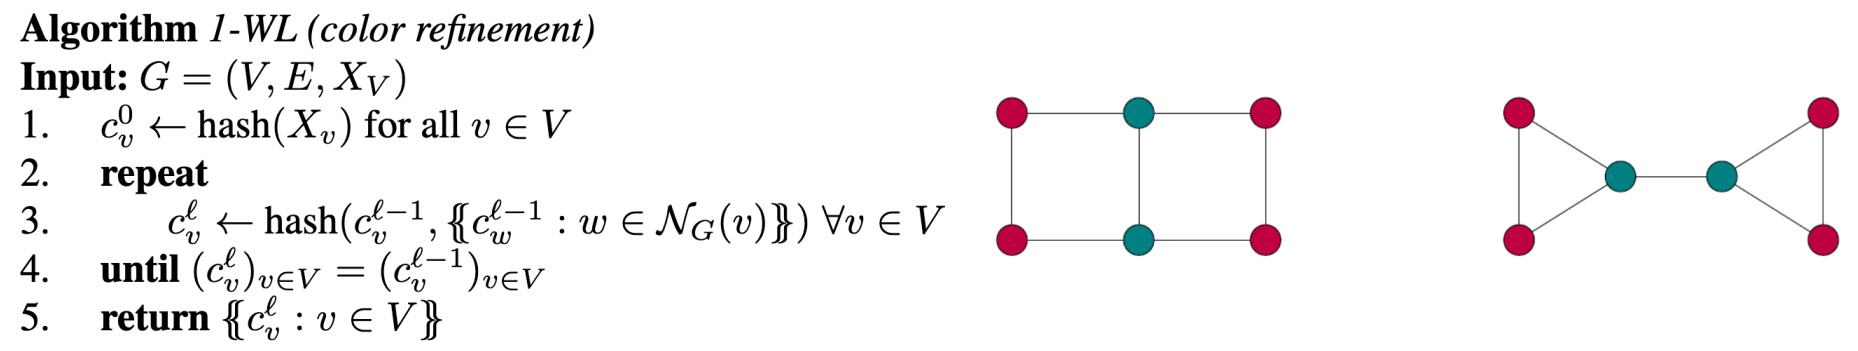
\includegraphics[width =\linewidth]{contents/imgs/1-wl.png}
1-WL cannot distinguish these two graphs and neither can GNNs

\subsection{Exercises}
Let \(\mathcal{G}\) denote the group acting on the doman \(\Omega\) and let \(\chi(\Omega)\) denote the signals defined on \(\Omega\).\\
\(\mathcal{G}\)-\textbf{equivariance:} A function \(f\) is \(\mathcal{G}\)-equivariant if \(f(g\cdot x)=g\cdot f(x)\quad \forall x\in \chi(\Omega),\forall g\in \mathcal{G}\), where \(g\cdot x\) denotes the action of the group element g on the signal \(x\in \chi(\Omega)\). The action \(g\) on \(x\) can be written as \(\rho(g)x\), where \(\rho(g)\) is referred to as the group representation of \(g\) (typically \(\rho(g)\in \mathbb{R}^{n\times n} \text{ if } x\in \mathbb{R}^n\). For any \(h,g\in \mathcal{G}, \rho(hg)=\rho(h)\rho(g)\)


\(\mathcal{G}\)-\textbf{convolution:} The \(\mathcal{G}\)-convolution operator between two signals \(x, \theta\in \chi(\Omega)\) is a function of the group elements defined as \((x*\theta)(g)=\langle x, \rho(g)\theta\rangle_{\chi(\Omega)}=\int_{\Omega} x(u)\theta(g^{-1}u)du\), where \([\rho(g)\theta](u)=\theta(g^{-1}u)\). Substituting in \(\mathcal{G}\) the cyclic shift group \(\mathcal{G}=\mathcbb{Z}_n=\{0,\ldots, n-1\}\) and \(\Omega=\mathbb{Z}_n\), we get back the 1D convolution.\\
\textbf{Theorem} The \(\mathcal{G}\)-convolution is \(\mathcal{G}\)-equivariant:
\((\rho(h)x*\theta)(g)=\langle\rho(h)x, \rho(g)\theta)\rangle_{\chi(\Omega)}=\int_{\Omega} x(h^{-1}u)\theta(g^{-1}u)du \stackrel{h^{-1}u=z}{=}\int_{\Omega}x(z)\theta((h^{-1}g)^{-1}z)dz=(x*\theta)(h^{-1}g)=[\rho(h)(x*\theta)](g)\)\\
\textbf{Permutation Equivariance:} Let \(\phi:\mathbb{R}^D\rightarrow \mathbb{R}^{D^\prime}\) be a function of a node and its neighbourhood. A permutation \emph{equivariant} function can be cast in the form \(f(X, A) = [\phi(x_1, X_{\mathcal{N}_1}), \ldots, \phi(x_N, X_{\mathcal{N}_N})]\) as long as \(\phi\) is permutation \emph{invariant} (e.g. sum, mean, maximum). This generally can be proven by letting \(\{i_1, i_2, \ldots i_N\}\) be the set of permuted indices \([i_1, i_2, \ldots, i_N]=[1,2, \ldots N]P\): \(f(XP, PAP^\top)=[\phi(x_{i_1}, X_{\mathcal{N}_{i_1}}), \ldots, \phi(x_{i_N}, X_{\mathcal{N}_{i_N}})]=([\phi(x_{i_1}, X_{\mathcal{N}_{i_1}}), \ldots, \phi(x_{i_N}, X_{\mathcal{N}_{i_N}})]P^\top)P=[\phi(x_1, X_{\mathcal{N}_1}), \ldots, \phi(x_N, X_{\mathcal{N}_N})]P=f(X,A)P\)\\
\textbf{Dirichlet Energy:} The Dirichlet energy \(E\) of a signal \(x\) on a graph is defined as \(E(x)=\frac{1}{2}\sum_{u,v} A_{uv}(x_u-x_v)^2=x^\top L x\), where \(L\) is the graph Laplacian and hence \(\frac{\partial^2E(x)}{\partial x^2}=L\) (also implies $L$ is psd) 